\section{Methodology}\label{sec:methodology}
Integrating runtime verification with DTs requires connecting concrete \emph{instance(s)} of the DT and concrete instance(s) of the RV monitor.
These twin and monitor instances must be generated, managed, and linked within the platform, DTaaS, throughout their lifetime.
Consequently, RV tool providers aiming for adoption within the DT community must understand the various approaches available for integrating the monitors, to ensure their tools are accessible and usable to the DT community.
In this section, we present different ways of creating DTs and integrating the monitors into DTs.


\subsection{The Digital Twin Assets and Lifecycle Phases}
\label{sec:dt-integration}

Each DT asset, that is managed inside DTaaS, is a reusable component falling into one of the following categories:
\begin{description}
	\item[Data:] a DT asset that provides data from the PT (a data source) or consumes data (a data sink) from a DT. The data asset can have its origins in two different places. The first source of data is PT which can either be a real one, or a mock. The mock PTs help with the DT development. The second source of data is the environment in which PT operates. Similar to PT, the environment data can come from sensing the environment around PT or a mock version of the environment.
	\item[Model:] describes the physical behavior of the PT. The models can be physics-based, numerical, data-driven, co-simulation, or a combination thereof. Both PT and DT will have their models. While the PT models are used for product development, DT models are used for instantiating digital replicas of the PT. It is advantageous to use the same model for both PT and DT but is often not possible primarily due to: 1) the lack of availability of the same model among all users, 2) divergent technical needs needing different models, 3) modeling software not being able to create models usable inside DTs.
	\item[Tool:] a software tool that can be used to create, evaluate, and analyze a model. Tools tend to be more reusable than models. For example, software tools such as Matlab\footnote{\url{https://mathworks.com}} can generate and evaluate models of different types (physics, numerical, co-simulation, etc.). The tools can also be used to perform in-time generation of models. In this case, the actual DT models are generated from a model configuration file when the DT is about to be executed. Some of the RV tools fit into this category because these RV tools generate monitoring at the start of executing DT.
	\item[Service:] provides a well-defined functionality over inter-process communication or computer network. Each service runs as one or more operating system processes accessible over an application programming interface (API). A service is reusable by all eligible consumers of that service. Within the context of DTs, services are used to satisfy concurrency and external integration needs. A DT performing run-time monitoring might send alerts to users or other external services (such as quality control audit software).
\end{description}%
%
\begin{figure}[]
	\centering
	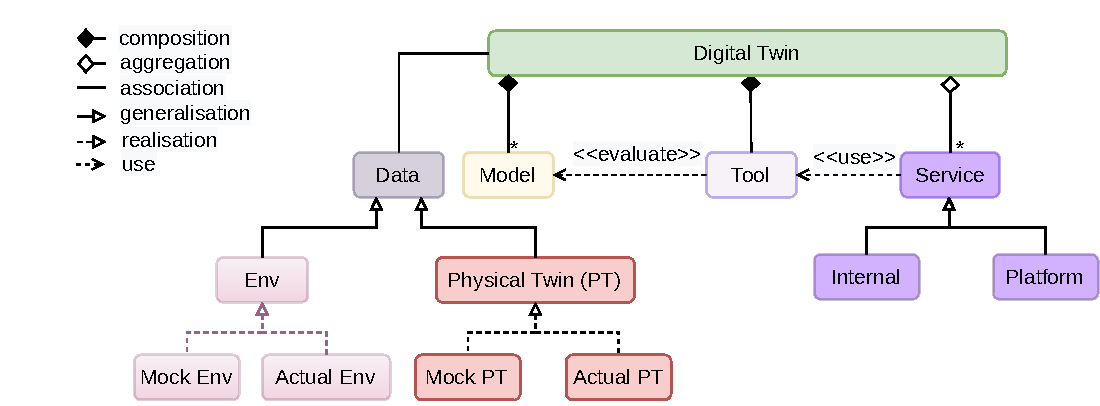
\includegraphics[width=1.0\textwidth]{images/assets-relationship.pdf}
	\caption{A class diagram for DT. The diagram illustrates the composition of data, models, tools, and services to form a DT.}
	\label{fig:dt-class-diagram}
\end{figure}%
%
\cref{fig:dt-class-diagram} shows a class diagram of DT. The four types of reusable assets - data, models, tools, and services - are shown as separate classes. Each class has properties that need to be defined at the DT instantiation time. For example, a data source conforming to MQTT protocol needs to have the MQTT broker access details. Here the access details are the properties of the data class. Similarly, models might have initial values, services will have service definitions/configurations and tools will have configurations. The DTaaS platform provides templates for supplying properties to DT and all assets used in it. A DT asset provider needs to provide the configuration template in which the properties can be filled.
The DT creator creates a DT-level configuration template and creates a configuration program/script whose primary responsibility is to translate the top-level DT class properties (configuration values) to asset-level properties. The DT users update the configuration values to create DT instances and link them with PTs.
The RV tool providers need to provide configuration templates for their RV tools so that the DT creators can translate the DT properties to the configuration values of their RV tools.
%\morten{Perhaps, this can come earlier to follow a more top-down approach.}\prasad{Explaining RV config with explaining the need for config seems confusing. Perhaps I can use example configs from section 4 in a table to illustrate the type of configs RV providers can use.}

It is important to remember that the class relationships shown in the \cref{fig:dt-class-diagram} can follow all variations of class associations. The actual class relationships shown in the figure reflect the examples being presented in this tutorial. The DT has an association type relationship with data coming from both PT and its environment. The DT class has composition type of relationship with Model, and Tool classes. The services are only aggregated by the DT class. In the case of services that are reusable simultaneously across multiple DTs, aggregation is the most appropriate class relationship. Similarly, in the case of any assets whose instances are only used exclusively within a DT, the relationship necessarily is that of composition. The models and tools need to be instantiated uniquely for each DT and thus they both tend to have composition type relationship with their DTs.
In addition, there is also a dependency relationship between the assets themselves, especially among services and tools. Some tools can also be run as services which will be showcased in the examples below.

A PT goes through multiple lifecycle phases [Ref...] necessitating the support for lifecycle phases within DTs. Certain research communities use design-manufacture-operate-recycle phases as representative lifecycle phases for a PT [Ref...]. This tutorial illustrates the use of RV tools on DTs during the operational phase. Thus only the \emph{create}, \emph{execute} and \emph{terminate} lifecycle phases are being illustrated. Two different kinds of activities are undertaken in the create phase: 1) creation of models, monitors if any 2) creation of execution environment by installing the necessary dependencies.
The execution phase includes the instantiation of DT and its use. The DT is available for interaction and the monitors are active in this phase. Finally, the terminate phase includes the termination of DT execution and revocation of all resources allocated to the terminated DT.


\subsection{General Techniques for Monitor Integration}
Several approaches exist for integrating RV monitors into DTs, dependent upon the capabilities of the underlying RV tool.%\prasad{Only the NuRV generates monitors. The TeSSLa takes monitoring properties and works as is without generating a separate monitor.}
Consequently, certain monitors may offer greater flexibility and require less effort to integrate from the perspective of DT developers.
Regardless of the approach, a monitor instance must be established and linked to each twin instance (DT asset) for monitoring individual properties.
The differentiating factor lies in whether the monitor is exposed as a service and who manages its lifecycle.
We distinguish the following approaches:%
%
\begin{description}
	\item[\methodone:] The RV tool, below just called ``tool'', is published as a reusable asset for the platform that generates a monitor instance used within a twin instance.
		%\prasad{"The tool" is being used to mean RV tool. There is also another kind of tool that is used for executing models. It is probably best to make this distinction upfront.} clarified
		The tool merely generates the monitor instance, which afterward is completely inside the twin instance, meaning their life cycles are tied together.
		%\prasad{there is no dedicated monitor instance} reworded
	\item[\methodtwo:]
		The tool is published as a reusable service that is instantiated from a twin instance.
		Each twin instance manages its monitor instance as an internal service.
	\item[\methodthree:]
		The tool is published as a reusable service that is instantiated and managed outside of twin instances.
		The twin instance uses it as an external service.
		When the twin instance finishes, the monitor service continues to be active. Any future twin instances can reuse the same external service.
\end{description}

In the following, we describe each possibility in detail before providing a guide on deciding which approach to take.

\subsubsection{Runtime Verification as a \methodone}
In this scenario, the RV tool is invoked to generate the monitor when the twin instance is created -- once for each property that the twin instance requires to be monitored.
Each invocation creates one reusable monitor, which is packaged as a binary, for example, a Functional Mock-Up Unit.\prasad{FMUs contain more than binaries. Perhaps a better word?} \morten{Open to suggestions. Must also be changed further down then}\prasad{can't think of any. Perhaps we just keep the existing text.}
The binary is then sent to the twin instance -- it is the task of the twin instance to integrate the monitor instance into its application.

As a consequence, the platform itself is unaware of the monitor instance -- it is handled completely within the twin instance -- which makes this option the most lightweight when it comes
to extending the platform. Concerning the twin instance itself, however, it requires a tight coupling between the platform tool and monitor instance --
changing the application may require changing the platform tool.
Similarly, as the platform is unaware of the monitor instance, it must be handled by the twin instance during shutdown.
In particular, its results, e.g., violation logs, must be stored.

%You are right about the mix-up of terms. I made the mistake of not labeling the DT assets correctly. We should use the following DT assets:
%Data, Models, Tools, Functions and Services
%
%The patterns may be explained as follows.
%
%    RV is published as a reusable tool takes a model input and generates a model used to be used within DT. In this, a model asset is converted to another model just-in-time and then DT is run. NuRV is an example of this scenario.
%    RV is published as a reusable service and is used inside DT as a service. I think we can keep RVs as services and then integrate them into DT. The service remains active only when the DT is active. Tessla as implemented in firefighter use case is an example of this scenario.
%    RV is published as a platform service and is used inside DT as a service. In this scenario, the service is always available an active DT uses the platform service. I am told that Tessla can work in this mode but we don't have an example for this scenario.
%
%
%The second is a reuse of the following
%
%    Same RV properties used with different RV tool/service in same or different DTs. In this case, a DT configuration can select an RV tool.
%    Different RV properties are used with one RV tool/service. In this case, RV properties are specified in the DT configuration, and the RV tool runs with the selected RV property.
%
%We don't have examples of this kind of reuse.
%
%The diagrams need to be corrected by changing the terms. I hope the explanation is clear.


\subsubsection{Runtime Verification as an \methodtwo}
In this scenario, the RV tool generates the monitor as an internal service, that is started and stopped alongside the twin instance.
The twin instance, once started, provides the property to the RV tool and then connects to the newly started RV service. Potential advantages are:
\begin{enumerate}
	\item decoupling of RV tool deployment
	\item possibility of defining RV properties from DTs
	\item possibility of creating multiple instances of an RV service (one per DT)
\end{enumerate}%
%
As a consequence, the twin instance manages the monitor service instance; for example, its start and shutdown must be managed in the twin instance.
The twin instance has a clear interface to interact with the internal monitor service and, thus, is potentially less tightly coupled,
as the interface can abstract away from all details except for data exchange.

\subsubsection{Runtime Verification as an \methodthree}
In this scenario, the RV monitor exists as an external service to the twin instances. This means multiple twin services can use the same monitoring service and each twin instance can interact with its coupled monitor instance through an API.
As a consequence, this approach completely decouples the twin and monitor instances, with all logic related to the monitor instance managed independently.
The twin instance continues to utilize a clear interface, while the monitor instance can be subjected to fine-grained control beyond the possibilities of general workflows within each twin instance.
However, this necessitates a separate implementation of all lifecycle management for the RV service, potentially leading to redundancy with features already present either within separate twin instances or the platform services.

%\prasad{Can the purpose be placed after the discussion?} no, the discussion is in light of the purposes
\subsubsection{Purposes}
Integrating a monitor can serve several purposes in a DT, and we briefly discuss the most relevant. The purpose must be considered when choosing the integration approach.
It is out of the scope of this tutorial to discuss all possible uses of RV, and we focus on three groups: Interaction, target structure of the monitor, and target concept of the monitor.

For interaction, the purpose of the monitor instance is to target different levels of interactions with the twin instance.
On one extreme, it may merely \emph{report}, i.e., run alongside the twin instance and output a warning or summary to the user without influencing the behavior or structure of the twin instance.
Conversely, the output of a monitor instance can be used directly to \emph{control} the PT from the twin instance.
In between, the monitor instance can act as a  shield~\cite{DBLP:conf/tacas/BloemKKW15}, i.e., manipulate the data streams between PT and DT to ensure some property without being a complete controller.

We stress that this discussion is orthogonal to the classification of a system as digital shadow or DT~\cite{KRITZINGER20181016} -- if the monitor instance is used as a reporting tool, the overall system may still be a DT, as other components may implement the control loop.

For the target structure and concept, the monitor instance is monitoring some stream of data. This can either be from the PT, i.e., monitoring sensor streams, the DT itself, i.e., monitoring control streams, or their combination, i.e., or the \emph{interconnection} between the PT and DT.

Finally, the monitor instance can monitor \emph{behavior}, or it can monitor \emph{structure}, where monitoring structure does not influence the control and data streams between the PTs and DTS, but the internal composition of the twin instance -- which may be connected to the PT via an asset model or similar~\cite{DBLP:conf/isola/KamburjanKSTCJ22}.


\subsubsection{Discussion}
RV tool providers must consider which of the approaches they wish to support with their generated monitors.
Supporting the \methodone\ approach provides a tight coupling between the monitor and twin instances, which makes this integration more accessible at the cost of manual handling of the tool lifecycle for the user.
The implementation effort for this approach is relatively low, as the tool instance only generates a binary.
Supporting the \methodtwo\ approach gives a looser coupling, which provides more flexibility (as it enforces a specific lifecycle and interface) but neither requires the user nor the DT developer to handle the lifecycle.
Supporting the \methodthree approach, in contrast to \methodtwo, gives the DT developer more flexibility, as they can improve the management of multiple monitor instances through more precise lifecycle management.

Finally, the purpose must be considered. Tight interaction, such as control, benefits from the flexibility of service integration, while loose interaction can be realized with less effort on the development side. Regarding the target, a platform service may perform some optimization if several services are using monitor instances for the same PT. Finally, structural monitoring and reconfiguration are easier to realize if the structure of the twin instance is easily available, i.e., it is a platform tool integration.

% \Cref{fig:choice} gives an overview of the trade-off without considering the purpose.
%\begin{table}[]
%\begin{tabular}{l|llll}
%                 & effort (user) & effort (integration) & flexibility (user)       & flexibility (integration) \\ \hline
%Platform Tool    & high          & low                  & high                     & low                       \\
%Reusable Serv.\ & low           & low                  & low                      & low                       \\ 
%Platform Serv.\ & low           & high                 & low & high 
%\end{tabular}
%    \caption{Overview over the flexibility-effort trade-off}
%\label{tab:choice}
%\end{table}


%\lars{a diagram like Fig.~\ref{fig:choice} might be easier to grasp than a table; @Eduard do you think the reduction to two dimensions fits the problem?}\prasad{the graph is better and is an equivalent representation to table.}

% \begin{figure}
% 
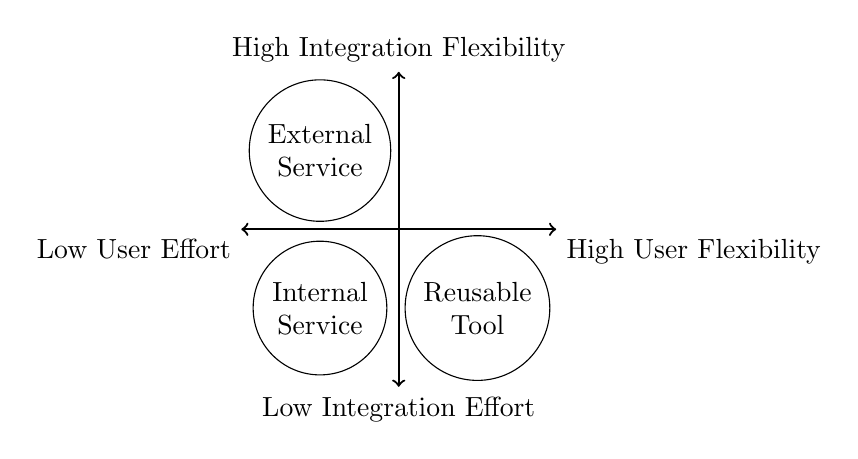
\begin{tikzpicture}[scale=1, every node/.style={scale=1}]

    % Draw axes
    \draw[thick,->] (0,0) -- (2,0) node[anchor=north west] {High User Flexibility};
    \draw[thick,->] (0,0) -- (0,2) node[anchor=south ] {High Integration Flexibility};
    \draw[thick,->] (0,0) -- (-2,0) node[anchor=north east] {Low User Effort};
    \draw[thick,->] (0,0) -- (0,-2) node[anchor=north ] {Low Integration Effort};

    % Add the three combinations
    % Reusable Service: Low Integration Effort and Low User Effort
    \node[align=center, draw, circle] (RS) at (-1,-1) {Internal\\Service};

    % Platform Tool: Low Integration Effort and High User Flexibility
    \node[align=center, draw, circle] (PT) at (1,-1) {Reusable\\Tool};

    % Platform Service: Low User Effort and High Integration Flexibility
    \node[align=center, draw, circle] (PS) at (-1,1) {External\\Service};

\end{tikzpicture}


% \caption{Overview over the flexibility-effort trade-off}
% \label{fig:choice}
% \end{figure}

